\documentclass[border=4pt]{standalone}
\usepackage{amsmath,amssymb,tikz}
\usetikzlibrary{arrows.meta}
\definecolor{figB}{RGB}{31,90,166}\definecolor{figR}{RGB}{176,48,48}\definecolor{figG}{RGB}{46,125,50}\definecolor{figO}{RGB}{214,120,20}
\begin{document}
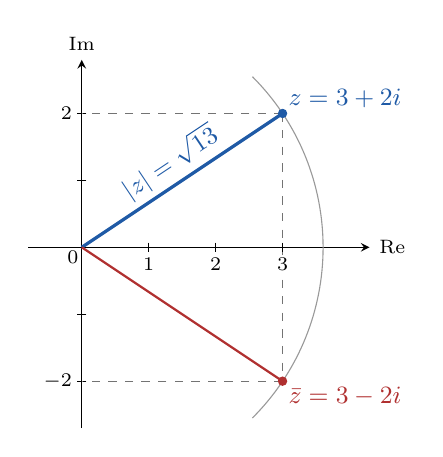
\begin{tikzpicture}[scale=0.85,>={Stealth[length=2mm]}]
\draw[thin,-stealth] (-0.8,0)--(4.3,0) node[right,font=\scriptsize]{$\operatorname{Re}$};
\draw[thin,-stealth] (0,-2.7)--(0,2.8) node[above,font=\scriptsize]{$\operatorname{Im}$};
\foreach \y in {-2,-1,1,2} \draw[thin] (0.07,\y)--(-0.07,\y);
\node[font=\scriptsize,below left,inner sep=1pt] at (0,0) {$0$};
\node[font=\scriptsize,left] at (0,2) {$2$}; \node[font=\scriptsize,left] at (0,-2) {$-2$};
% circle |w| = sqrt 13
\draw[black!40] ({sqrt(13)*cos(-45)},{sqrt(13)*sin(-45)}) arc (-45:45:{sqrt(13)});
% projections
\draw[dashed,black!55] (3,2)--(3,-2);
\draw[dashed,black!55] (3,2)--(0,2);
\draw[dashed,black!55] (3,-2)--(0,-2);
\foreach \x in {1,2,3} \draw[thin] (\x,0.07)--(\x,-0.07) node[below=1pt,font=\scriptsize,inner sep=1pt,fill=white]{$\x$};
% z and its conjugate
\draw[very thick,figB] (0,0)--(3,2) node[pos=0.5,above,sloped,font=\small,inner sep=2pt]{$|z|=\sqrt{13}$};
\draw[thick,figR] (0,0)--(3,-2);
\fill[figB] (3,2) circle (2pt) node[above right,font=\small,inner sep=2pt]{$z=3+2i$};
\fill[figR] (3,-2) circle (2pt) node[below right,font=\small,inner sep=2pt]{$\bar z=3-2i$};
\end{tikzpicture}
\end{document}
